\chapter{Federated Learning}

\section{Introduction to Federated Learning}

\subsection{Recap: Centralized Machine Learning}
Until now we have seen only a centralized machine learning that has some characteristics, that include:
\begin{compactitemize}
    \item \textbf{All data in one place}: Training data from alla sources is aggregated and stored on a central server or in a data center. The model has access to the entire dataset during training.
    \item \textbf{Single model, combined dataset}: A single global model is trained oh this unified dataset. This traditional approach relied on processing all data centrally before model training.
    \item \textbf{Iterative optimization (SGD)}:The model's parameters are iteratively updated using SGD, epoch after epoch until the model converges.
\end{compactitemize}

\subsection{Problems Motivating Decentralized and Federated Learning}

In many real-world scenarios, the traditional paradigm of \textbf{centralized machine
learning}—where all data are collected and stored on a single server—is either impractical
or undesirable. Several fundamental challenges motivate the need for decentralized and
federated learning approaches.

\begin{compactitemize}
    \item \textbf{Data privacy and confidentiality.}  
    Many application domains involve \textbf{sensitive data}, such as personal information,
    medical records, or financial transactions. Transferring these data to a central server
    raises serious privacy risks and increases exposure to data breaches. In such settings,
    data should ideally \textbf{remain on-device or on-premise}, and only model-related
    information should be shared.

    \item \textbf{Bandwidth limitations and data scale.}  
    Modern datasets are often extremely large, making data centralization costly or
    infeasible. Uploading raw data from millions of edge devices would require enormous
    communication bandwidth and incur high latency. In contrast, sharing compact model
    updates is significantly more efficient.

    \item \textbf{Exploiting distributed computational resources.}  
    Edge devices such as smartphones, IoT devices, and local servers possess substantial
    computational power. Decentralized learning frameworks allow these clients to perform
    most of the computation locally, reducing the load on central servers and enabling
    better scalability.

    \item \textbf{Regulatory and legal constraints.}  
    Data protection regulations such as \textbf{GDPR}, \textbf{HIPAA}, and similar legal
    frameworks impose strict constraints on how data can be stored, processed, and shared.
    Keeping data localized while exchanging only model updates helps ensure compliance with
    these regulations.
\end{compactitemize}

Together, these challenges highlight the limitations of centralized learning and motivate
learning paradigms in which \textbf{data remain decentralized}, while models are trained
collaboratively across multiple clients. This setting naturally leads to approaches such as
\textbf{Federated Learning}, which aim to balance privacy, efficiency, and scalability.

\subsection{Solution: Federated Learning}

\textbf{Federated Learning (FL)} is a distributed machine learning paradigm designed to
address the limitations of centralized training in privacy-sensitive and large-scale
settings. In Federated Learning, a \textbf{central server} coordinates a population of
\textbf{clients} (e.g., mobile devices, hospitals, companies) to collaboratively train a
shared model \textbf{without collecting or centralizing raw data}.

Each client keeps its local dataset private and performs training locally. Only
\textbf{model updates}—such as weights or gradients—are communicated to the server, which
aggregates them to form a global model. This approach enables learning from decentralized
data while improving privacy, reducing communication costs, and exploiting distributed
compute resources.

\textbf{Key idea:} \emph{keep data local, share only model updates.}
\begin{figure}[H]
    \centering
    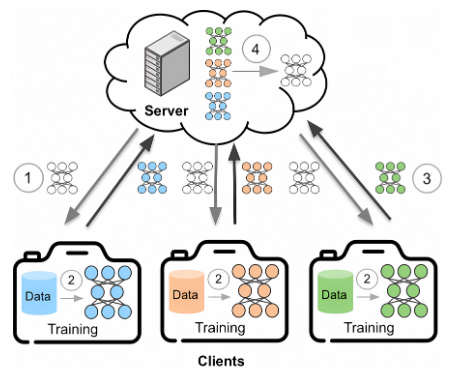
\includegraphics[width=0.5
    \textwidth]{images/FL1.png}
    \label{fig:MHA2}
\end{figure}

\vspace{0.3cm}

\begin{center}
    \hrule
    \vspace{0.3cm}
    
    \begin{minipage}[t]{0.47\textwidth}
    \centering
    \textbf{Client-side Objective}
    
    \vspace{0.2cm}
    \hrule
    \vspace{0.2cm}
    
    Each client $i$ holds a private dataset $D_i$.  
    The client optimizes its local model parameters $\theta_i$ by minimizing the loss
    using only its own data:
    
    \[
    \min_{\theta_i}
    \;
    \mathbb{E}_{(x,y)\sim D_i}
    \bigl[
    \mathcal{L}\bigl(f_{\theta_i}(x), y\bigr)
    \bigr].
    \]
    
    \vspace{0.15cm}
    
    Local training is performed independently and no raw data are shared with the server
    or other clients.
    
    \end{minipage}
    \hfill
    \begin{minipage}[t]{0.47\textwidth}
    \centering
    \textbf{Server-side Objective}
    
    \vspace{0.2cm}
    \hrule
    \vspace{0.2cm}
    
    The server has \textbf{no access to data}. Its goal is to obtain a global model
    $\theta$ that minimizes the average loss across all $N$ clients:
    
    \[
    \min_{\theta}
    \;
    \frac{1}{N}
    \sum_{i=1}^{N}
    \mathbb{E}_{(x,y)\sim D_i}
    \bigl[
    \mathcal{L}\bigl(f_{\theta}(x), y\bigr)
    \bigr].
    \]
    
    \vspace{0.15cm}
    
    This objective is achieved by aggregating local updates received from the clients.
    
    \end{minipage}
    
    \vspace{0.3cm}
\hrule
\end{center}

\vspace{0.3cm}

This formulation highlights the fundamental asymmetry of Federated Learning: \textbf{clients
optimize locally using private data}, while the \textbf{server coordinates and aggregates}
without ever observing raw samples. As a result, FL provides a principled solution to
privacy, scalability, and regulatory challenges in modern distributed learning systems.

\subsection{Application Scenarios}

Federated Learning can be applied in different real-world settings depending on the number
of participating clients and the characteristics of their local datasets. Two main
application scenarios are commonly distinguished.

\begin{compactitemize}
    \item \textbf{Cross-device Federated Learning.}  
    This scenario involves a \textbf{massive number of edge devices}, such as smartphones,
    wearables, or IoT sensors. Each device typically holds only a \textbf{small amount of
    data}, and participation is often intermittent due to connectivity or energy
    constraints.  
    A canonical example is training a \textbf{mobile keyboard or language model} directly
    on users’ phones, where sensitive information such as keystrokes remains on-device and
    is never uploaded to a central server.

    \item \textbf{Cross-silo Federated Learning.}  
    In this setting, the number of clients is relatively \textbf{small}, but each client
    (or silo) owns a \textbf{large and rich local dataset}. Typical clients include
    organizations such as hospitals, banks, or research institutions.  
    A representative example is multiple \textbf{hospitals collaboratively training a
    medical diagnostic model} without sharing patient records, thereby preserving privacy
    and complying with data protection regulations.
\end{compactitemize}

These two scenarios differ significantly in scale, communication patterns, and system
constraints, but both share the core principle of Federated Learning: \textbf{collaborative
training without data centralization}.

\subsection{Weight Averaging and Model Merging}

A fundamental mechanism underlying Federated Learning is \textbf{weight averaging}, also
referred to as \textbf{model merging}. This procedure enables a central server to improve a
global model by aggregating locally trained models, even though it has \textbf{no access to
any training data}.

The federated training process proceeds iteratively as follows:

\begin{enumerate}
    \item \textbf{Initialization.}  
    The server initializes a global model $\theta^{(0)}$. The server holds \textbf{no data},
    as all training samples are distributed across the clients.

    \item \textbf{Broadcast.}  
    At each communication round, the server selects a subset of clients and \textbf{sends
    the current global model} to them.

    \item \textbf{Local training.}  
    Each selected client performs local optimization on its private dataset for one or more
    epochs, obtaining an updated set of parameters based solely on local data.

    \item \textbf{Upload of updates.}  
    After local training, clients \textbf{send their model updates}—such as gradients or
    updated weights—back to the server.

    \item \textbf{Aggregation.}  
    The server \textbf{aggregates the received updates}, typically by computing a weighted
    or unweighted average, to obtain an improved global model.

\end{enumerate}

These steps are repeated until convergence. Through repeated rounds of local training and
global aggregation, the server progressively refines the global model without ever
observing raw client data.


\subsection{Key Challenges in Federated Learning}

Despite its advantages, Federated Learning introduces a number of fundamental challenges
that distinguish it from standard centralized training.

\begin{compactitemize}
    \item \textbf{Data heterogeneity (non-IID data).}  
    Clients typically possess data drawn from \textbf{different and potentially skewed
    distributions}. This non-IID setting can lead to \textbf{client drift}, where local
    updates move model parameters in conflicting directions, often resulting in slower
    convergence and reduced global accuracy.

    \item \textbf{Partial participation.}  
    In each communication round, only a \textbf{subset of clients} is available or willing
    to participate. The active client set may change across rounds due to stragglers,
    drop-outs, or connectivity constraints, introducing instability in the training
    process.

    \item \textbf{Communication overhead.}  
    Communication is often the main bottleneck in FL. Limited network capacity and high
    latency make it crucial to \textbf{minimize the size and frequency of model updates}
    exchanged between clients and the server in order to achieve efficient training.

    \item \textbf{Privacy and security.}  
    Although raw data remain local, \textbf{model updates can still leak sensitive
    information}. Adversarial attacks such as gradient inversion or membership inference
    highlight the need for additional privacy-preserving and security mechanisms.
\end{compactitemize}

Addressing these challenges is essential for making Federated Learning robust, scalable,
and deployable in real-world environments.

\section{Federated Averaging (FedAvg)}

\textbf{Federated Averaging (FedAvg)} is the foundational algorithm for Federated Learning,
introduced by McMahan et al.\ It provides a simple yet effective strategy for training a
global model from decentralized client updates.

At each communication round, the server selects a subset of clients and sends them the
current global model. Each selected client trains the model locally using its private data
for a fixed number of epochs and then returns the updated model parameters to the server.
The server combines these updates to obtain a new global model. This iterative procedure
is repeated over multiple rounds until convergence.

The key question addressed by FedAvg is:

\begin{center}
\emph{How should client updates be combined to form an improved global model?}
\end{center}

FedAvg answers this question using a \textbf{weighted averaging scheme}, where each
client’s contribution is proportional to the size of its local dataset. In this way,
clients with more data have a stronger influence on the global model, better approximating
the objective of minimizing the average loss across all clients.

\subsection{FedAvg Algorithm}

\vspace{0.3cm}

\noindent\rule{\textwidth}{0.8pt}

\noindent\textbf{Initialize:}  
Server initializes global model parameters $w_0$.

\noindent\textbf{for} communication rounds $t = 1, 2, \dots, T$ \textbf{do}

\noindent\hspace{0.6cm}\textbf{Client selection:}  
\noindent\hspace{0.6cm}Server selects a subset $C_t$ of available clients.

\noindent\hspace{0.6cm}\textbf{Broadcast:}  
\noindent\hspace{0.6cm}Server sends the current global model $w_{t-1}$ to all clients in $C_t$.

\noindent\hspace{0.6cm}\textbf{Local training:}  
\noindent\hspace{0.6cm}Each client $i \in C_t$ initializes its local model with $w_{t-1}$ and
performs local optimization (e.g., $E$ epochs of SGD) on its private dataset to obtain
updated parameters $w_t^{\,i}$.

\noindent\hspace{0.6cm}\textbf{Upload:}  
\noindent\hspace{0.6cm}Each client sends its updated model parameters $w_t^{\,i}$ (or the
model difference) back to the server.

\noindent\hspace{0.6cm}\textbf{Aggregation:}  
\noindent\hspace{0.6cm}Server aggregates the client models to form the new global model:
\[
w_t
\leftarrow
\sum_{i \in C_t}
\frac{n_i}{\sum_{j \in C_t} n_j}
\,
w_t^{\,i},
\]
where $n_i$ denotes the number of training samples at client $i$.

\noindent\textbf{end for}

\noindent\rule{\textwidth}{0.8pt}

\vspace{0.3cm}

Through repeated rounds of local training and weighted aggregation, FedAvg approximates
centralized empirical risk minimization while preserving data locality and privacy.

\subsection{FedAvg: Take-Home Message}

Federated Averaging works well when client data are approximately \textbf{i.i.d.} and has
become the \textbf{de facto baseline} for federated learning experiments.

\textbf{Strengths}:
\begin{compactitemize}
    \item \textbf{Simplicity}: FedAvg is easy to implement and requires minimal coordination
    between clients and server.
    \item \textbf{Communication efficiency}: multiple local SGD steps are performed before
    synchronization, significantly reducing communication frequency compared to fully
    synchronized distributed SGD.
\end{compactitemize}

\textbf{Limitations}:
\begin{compactitemize}
    \item \textbf{Sensitivity to non-IID data}: when client data distributions differ
    substantially, local models may drift toward different regions of the parameter space.
    \item \textbf{Client drift}: if local gradients point toward \emph{different directions},
    their average may no longer represent a meaningful descent direction for the global
    objective, harming convergence and final accuracy.
\end{compactitemize}

Intuitively, when gradients trend toward incompatible directions in the parameter space,
\textbf{simple averaging becomes ineffective}. As a consequence, the aggregated model may
fail to improve—or may even degrade—global performance.

These limitations have motivated a large body of work proposing \textbf{enhancements to
FedAvg}. Common strategies include modifying the local objective with additional
regularization terms (e.g., proximal constraints) or improving the aggregation procedure.
Next, we discuss the main families of approaches developed to address these challenges.

\subsection{Possible Improvements over FedAvg}

The limitations of FedAvg in heterogeneous settings have led to a variety of improved
federated learning methods. These approaches can be broadly categorized into three main
families.

\begin{compactitemize}
    \item \textbf{Server-side approaches.}  
    The server employs more sophisticated aggregation strategies instead of simple averaging.
    These methods aim to better align client updates or correct for bias introduced by
    heterogeneous data distributions.

    \item \textbf{Client-side approaches.}  
    Each client augments its local objective with additional terms—such as regularization or
    proximal constraints—that enforce \textbf{consistency with the global model}. This helps
    limit client drift during local training.

    \item \textbf{Prototype-based approaches.}  
    Constraints are enforced in \textbf{feature space} rather than directly in parameter
    space. By aligning class or representation prototypes across clients, these methods
    achieve a better trade-off between global consistency and local specialization.
\end{compactitemize}

These families of methods represent different ways of stabilizing federated optimization
under data heterogeneity, and form the foundation of many state-of-the-art federated
learning algorithms.

\section{Server-side Approach}

\subsection{Motivation for Fisher-Weighted Averaging}

Standard parameter averaging methods, such as \textbf{FedAvg}, treat every model parameter
as \textbf{equally informative}. Each weight dimension contributes uniformly to the
aggregation process, regardless of how important or reliable that parameter is for a
given client.

This assumption is reasonable when client updates are derived from \textbf{i.i.d. data}.
However, in federated settings with \textbf{data heterogeneity}, different clients may be
confident about different subsets of parameters. Uniform averaging can therefore be
sub-optimal, as it may dilute reliable parameters with noisy or conflicting updates.

\textbf{Key idea.}  
Instead of treating all parameters equally, the contribution of each model parameter should
be weighted by the \textbf{confidence} of the client in that parameter. This confidence can
be quantified using the \textbf{Fisher Information Matrix (FIM)}, which measures how
sensitive the model’s loss is to changes in each parameter.

By assigning higher weight to parameters with high Fisher information and lower weight to
less reliable ones, Fisher-weighted averaging aims to produce a global model that better
respects client-specific knowledge while remaining robust under heterogeneous data
distributions.


\subsection{Recall: Fisher Information Matrix}
\begin{wrapfigure}{r}{0.3\textwidth}
    \centering
    \vspace{-10pt}
    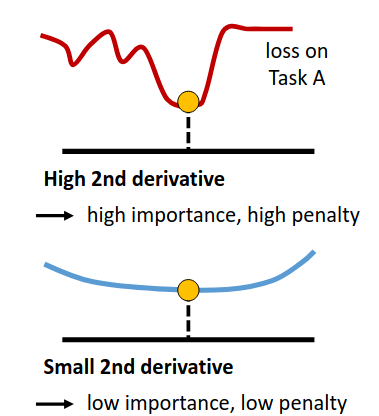
\includegraphics[width=\linewidth]{images/FL2.png}
    \label{fig:Scaled Dot Product Attention}
    \vspace{-10pt}
\end{wrapfigure}
One method previously discussed for estimating the importance of neural network parameters
is based on the \textbf{Fisher Information Matrix (FIM)}. The empirical Fisher Information
Matrix is defined as:
\[
F_\theta
=
\frac{1}{N}
\sum_{i=1}^{N}
\Bigl[
\nabla_\theta \log p\bigl(x^{(i)} \mid \theta\bigr)
\Bigr]
\Bigl[
\nabla_\theta \log p\bigl(x^{(i)} \mid \theta\bigr)
\Bigr]^{\top},
\]
where the gradients correspond to the derivatives of the loss function with respect to the
model parameters.

There exists a theoretical relationship between the empirical FIM and the \textbf{second
derivative of the loss function}. In particular, near a minimum, the Fisher Information
Matrix can be used as an approximation of the \textbf{Hessian matrix}.

Since the FIM captures the \textbf{local curvature} of the loss landscape:
\begin{compactitemize}
    \item a \textbf{high Fisher information} for a parameter indicates that the parameter is
    pivotal, and modifying it is likely to increase the loss;
    \item a \textbf{low Fisher information} indicates a flat region, meaning that small
    changes to the parameter have little effect on the loss.
\end{compactitemize}

\subsection{Fisher-Weighted Averaging: Core Formula}

Given $M$ client models $\{\theta_i\}_{i=1}^{M}$ with identical initialization, each client’s
posterior distribution is approximated as a Gaussian:
\[
p(\theta \mid \theta_i, F_i),
\]
where $F_i$ denotes the Fisher Information Matrix associated with client $i$.

The objective is to find the global model parameters $\theta^*$ that maximize the joint
posterior of all client models:
\[
\theta^*
=
\arg\max_{\theta}
\prod_{i=1}^{M}
\lambda_i \,
p(\theta \mid \theta_i, F_i),
\]
where $\lambda_i$ are scalar weights such that $\sum_i \lambda_i = 1$.

To simplify the optimization, all terms can be moved inside the logarithm:
\[
\theta^*
=
\arg\max_{\theta}
\sum_{i=1}^{M}
\lambda_i
\log p(\theta \mid \theta_i, F_i).
\]

This optimization problem admits a \textbf{closed-form solution}, given by:
\[
\theta^*
=
\left(
\sum_{i}
\lambda_i F_i
\right)^{-1}
\left(
\sum_{i}
\lambda_i F_i \theta_i
\right).
\]

\textbf{Practical considerations.}  
Estimating and storing the full Fisher Information Matrix is often infeasible for modern
neural networks due to their large number of parameters and over-parameterization.

A common solution is to use an \textbf{approximation of the FIM}, such as its diagonal. This
approximation can be represented as a vector and leads to a simplified aggregation rule:
\[
\theta^*
=
\frac{
\sum_{i=1}^{M}
\lambda_i F_i \theta_i
}{
\sum_{i=1}^{M}
\lambda_i F_i
}.
\]

This diagonal approximation makes Fisher-weighted averaging tractable in large-scale
federated learning settings.

\subsection{Practical Considerations in Federated Learning}

Fisher-weighted averaging introduces additional practical aspects that must be considered
when deploying the method in real federated learning systems.

\textbf{Computation of the Fisher Information.}  
The Fisher Information Matrix is typically computed \textbf{after each client finishes
local training}. In practice, only the \textbf{diagonal Fisher} is estimated, using the
squared gradients of the log-likelihood evaluated on a local mini-batch. This provides an
efficient approximation of parameter importance.

\textbf{Communication overhead.}  
Each client sends both the updated model parameters $\theta^{(k)}$ and the diagonal Fisher
$\mathrm{diag}(F^{(k)})$ to the server. Since both quantities are model-sized vectors, the
total communication payload is roughly doubled. However, this overhead is still practical
for typical federated learning models.

\textbf{Privacy considerations.}  
The Fisher Information Matrix does not reveal raw data, but only the \textbf{sensitivity of
the loss with respect to model parameters}. Nevertheless, it may still leak information.
For this reason, Fisher-weighted aggregation is often combined with \textbf{secure
aggregation} or \textbf{differential privacy} mechanisms.

\vspace{0.3cm}

The \textbf{strengths} of this approach are:
\begin{compactitemize}
    \item Improves accuracy over FedAvg on \textbf{heterogeneous data} by exploiting
    parameter importance.
    \item Tends to work particularly well when applied to \textbf{pretrained models} that
    share a common feature representation.
    \item Naturally supports \textbf{one-shot federated learning} or sporadic client
    participation, since models can be merged without requiring multiple communication
    rounds.
    \item Compatible with other \textbf{server-side techniques}, such as momentum or model
    quantization.
\end{compactitemize}

The \textbf{weaknesses} of this approach are:
\begin{compactitemize}
    \item Increased \textbf{client-side computation}, as multiple forward and backward
    passes are required to estimate the Fisher Information.
    \item Potential \textbf{numerical issues}, since the Fisher values may become very large
    or very small.
    \item Limited benefit when client models are \textbf{too far apart in parameter space},
    as the Fisher computed on local data may be meaningless when applied far from the local
    optimum.
\end{compactitemize}

\subsection{Derivation of Fisher-Weighted Averaging}
\begin{wrapfigure}{r}{0.4\textwidth}
    \centering
    \vspace{-10pt}
    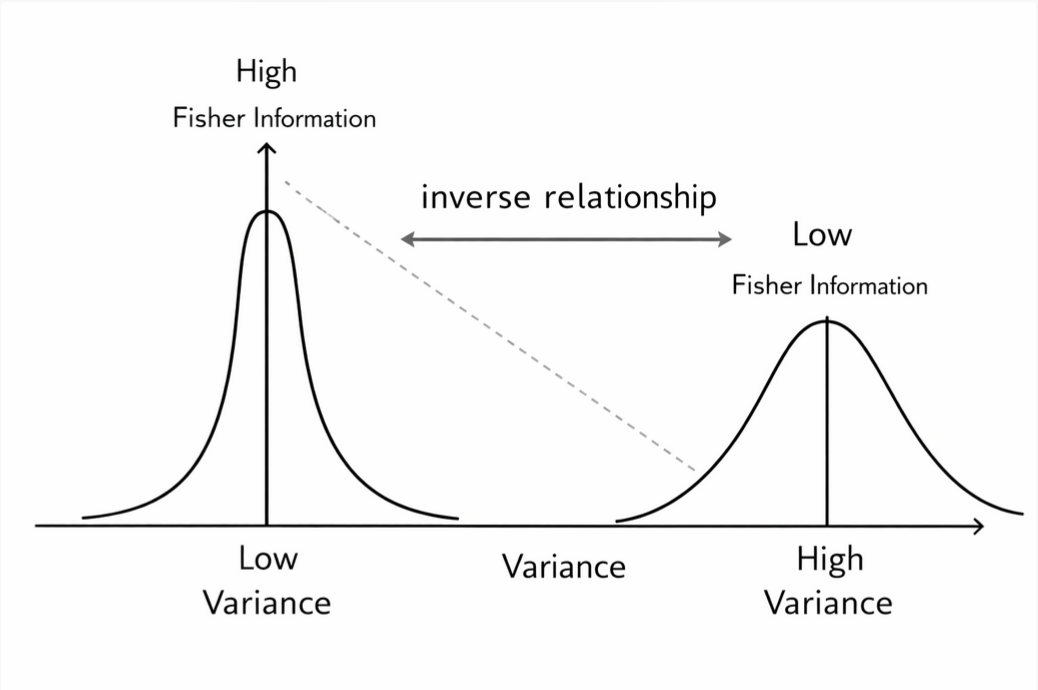
\includegraphics[width=\linewidth]{images/FL3.png}
    \label{fig:Scaled Dot Product Attention}
    \vspace{-10pt}
\end{wrapfigure}
\textbf{Setup.}  
After local training, each client $i = 1, \dots, M$ provides a parameter vector
$\theta_i \in \mathbb{R}^{n_p}$, where $n_p$ is the number of parameters of the network.
Each client also provides an estimate of parameter importance through the Fisher
Information Matrix $F_i \in \mathbb{R}^{n_p \times n_p}$, which is symmetric and positive
semi-definite.

We start by approximating the posterior distribution of each client as a Gaussian:
\[
p(\theta \mid \theta_i)
\;\approx\;
\mathcal{N}(\theta_i,\ \Sigma_i),
\]
where $\Sigma_i$ is the covariance matrix of the posterior around $\theta_i$.

Near a minimum, the inverse covariance can be approximated by the Fisher Information
Matrix:
\[
\Sigma_i^{-1} \;\approx\; F_i.
\]
As a result, the posterior can be rewritten as:
\[
p(\theta \mid \theta_i, F_i)
\;\approx\;
\mathcal{N}\bigl(\theta_i,\ F_i^{-1}\bigr),
\]
where $F_i$ acts as a \textbf{precision matrix}.  
Intuitively, a \textbf{low-variance posterior} corresponds to a \textbf{high Fisher
information} (high confidence), while a \textbf{high-variance posterior} corresponds to a
\textbf{low Fisher information} (low confidence).

The goal is to find the parameter vector $\theta^*$ that maximizes the joint posterior of
the $M$ independent client models:
\[
\theta^*
=
\arg\max_{\theta}
\prod_{i=1}^{M}
\lambda_i \, p(\theta \mid \theta_i, F_i),
\]
where $\lambda_i$ are scalar weights such that $\sum_i \lambda_i = 1$.

Taking the logarithm, this is equivalent to:
\[
\theta^*
=
\arg\max_{\theta}
\sum_{i=1}^{M}
\lambda_i \log p(\theta \mid \theta_i, F_i).
\]

\textbf{Gaussian form.}  
Since each posterior is Gaussian, the objective becomes:
\[
\theta^*
=
\arg\max_{\theta}
\sum_{i=1}^{M}
\lambda_i
\log
\left(
\exp\left\{
-\frac{1}{2}
(\theta - \theta_i)^\top
F_i
(\theta - \theta_i)
\right\}
\right).
\]

\textbf{Step 1 — Remove log and exponential.}  
Since $\log(\cdot)$ is monotone:
\[
\theta^*
=
\arg\max_{\theta}
-
\frac{1}{2}
\sum_{i=1}^{M}
\lambda_i
(\theta - \theta_i)^\top
F_i
(\theta - \theta_i).
\]

\textbf{Step 2 — Convert to minimization.}  
Multiplying by $-2$ yields the equivalent problem:
\[
\theta^*
=
\arg\min_{\theta}
\sum_{i=1}^{M}
\lambda_i
(\theta - \theta_i)^\top
F_i
(\theta - \theta_i).
\]

\textbf{Step 3 — Expand the quadratic forms.}
\[
\theta^*
=
\arg\min_{\theta}
\sum_{i=1}^{M}
\lambda_i
\Bigl(
\theta^\top F_i \theta
-
2 \theta^\top F_i \theta_i
+
\theta_i^\top F_i \theta_i
\Bigr).
\]
The last term does not depend on $\theta$ and can be removed from the optimization
problem.

\textbf{Step 4 — Collect terms.}
\[
\theta^*
=
\arg\min_{\theta}
\;
\theta^\top
\left(
\sum_{i=1}^{M} \lambda_i F_i
\right)
\theta
-
2
\theta^\top
\left(
\sum_{i=1}^{M} \lambda_i F_i \theta_i
\right).
\]

\textbf{Step 5 — Take the gradient and set it to zero.}  
Using symmetry of $F_i$:
\[
2
\left(
\sum_{i=1}^{M} \lambda_i F_i
\right)
\theta
-
2
\left(
\sum_{i=1}^{M} \lambda_i F_i \theta_i
\right)
= 0.
\]

\textbf{Step 6 — Solve for $\theta^*$.}
\[
\theta^*
=
\left(
\sum_{i=1}^{M} \lambda_i F_i
\right)^{-1}
\left(
\sum_{i=1}^{M} \lambda_i F_i \theta_i
\right).
\]

\textbf{Diagonal Fisher approximation.}  
If each $F_i$ is approximated by the diagonal of the Fisher Information Matrix, it can be
treated as a vector and the solution becomes element-wise:
\[
\theta^{*(j)}
=
\frac{
\sum_{i=1}^{M}
\lambda_i F_i^{(j)} \theta_i^{(j)}
}{
\sum_{i=1}^{M}
\lambda_i F_i^{(j)}
}.
\]

When all $F_i$ are identity matrices (i.e., all parameters are equally confident) and
$\lambda_i$ are proportional to the number of samples at each client, the solution reduces
to \textbf{standard weight averaging}, namely \textbf{FedAvg}.

\section{Client-Side Approach}
\subsection{The Client Drift Problem}
ith \textbf{non-i.i.d. data}, the local updates produced by different
clients may point toward \textbf{inconsistent directions}. This phenomenon is known as
\textbf{client drift} and represents one of the main limitations of FedAvg.

The core reason is that each client optimizes its model with respect to its \textbf{local
data distribution}. As a result, each client is driven toward its own local optimum, which
may differ significantly from the optimum of the global objective defined over all data.
Simply averaging these locally optimized models does not, in general, correspond to a
model obtained via joint training on the union of all datasets.
\begin{wrapfigure}{r}{0.4\textwidth}
    \centering
    \vspace{-10pt}
    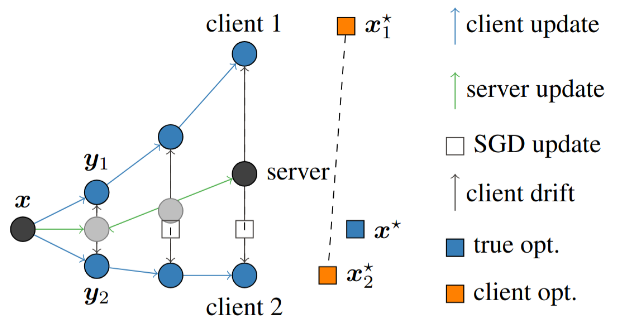
\includegraphics[width=\linewidth]{images/FL4.png}
    \label{fig:Scaled Dot Product Attention}
    \vspace{-10pt}
\end{wrapfigure}
In federated learning w
Client drift becomes increasingly severe as the data distributions across clients become
more \textbf{heterogeneous}. The problem is further exacerbated when only a \textbf{fraction
of clients participates} in each communication round, since the server observes a biased
and incomplete view of the global data distribution.

The consequence is often \textbf{slower convergence} or convergence to a
\textbf{suboptimal global model}. To address this issue, federated learning algorithms must
introduce mechanisms that better \textbf{align local updates with the global objective}.

\begin{infobox}[What do we mean by data heterogeneity in Federated Learning?]
    In Federated Learning, \textbf{data heterogeneity} refers to the fact that different clients
    observe data drawn from \textbf{different probability distributions}. Formally, each client
    $i$ has its own local data distribution $D_i$, and in general:
    \[
    D_1 \neq D_2 \neq \dots \neq D_M.
    \]
    
    This implies that:
    \begin{compactitemize}
        \item each client optimizes a \textbf{different local objective function};
        \item the \textbf{local optima} across clients may not coincide;
        \item the \textbf{gradients computed on different clients} may point in different
        directions.
    \end{compactitemize}
    
    As a result, when client data are heterogeneous (non-i.i.d.), averaging local updates does
    not approximate the update that would be obtained by training on all data jointly, leading
    to the \textbf{client drift problem}.
\end{infobox}
    
\subsection{Motivation: Simulating the Ideal Update}
\begin{wrapfigure}{r}{0.25\textwidth}
    \centering
    \vspace{-10pt}
    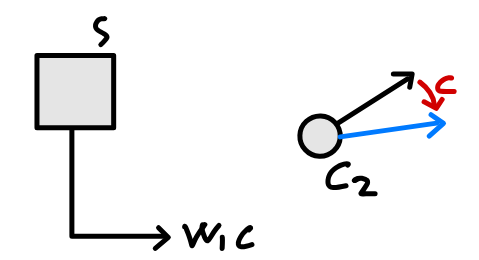
\includegraphics[width=\linewidth]{images/FL5.png}
    \label{fig:Scaled Dot Product Attention}
    \vspace{-10pt}
\end{wrapfigure}
The goal of many federated learning methods is to make each client follow, as closely as
possible, the \textbf{ideal update direction}. This ideal direction corresponds to the
update that would be obtained if \textbf{all data were available in a single place} and the
model were trained using standard centralized optimization.

Such an ideal update is easy to compute in settings where:
\begin{compactitemize}
    \item all training data are stored on a single client; or
    \item clients send both their \textbf{model parameters and gradients} to a central
    server.
\end{compactitemize}

In these cases, the server could aggregate all gradients, compute the global update
direction, and send it back to the clients. Each client would then use this information to
\textbf{correct its local update}, thereby avoiding the drift caused by non-IID data.

The main challenge is that \textbf{directly exchanging gradients is communication
expensive}, especially in large-scale federated systems. This motivates the need for
methods that \textbf{efficiently approximate the global correction} while maintaining low
communication overhead.

\subsection{SCAFFOLD}

\begin{wrapfigure}{r}{0.4\textwidth}
    \centering
    \vspace{-10pt}
    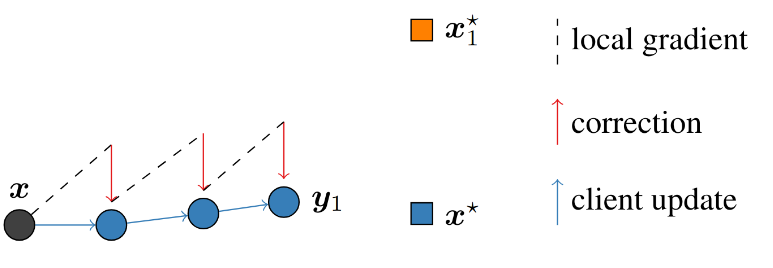
\includegraphics[width=\linewidth]{images/FL6.png}
    \label{fig:Scaled Dot Product Attention}
    \vspace{-10pt}
\end{wrapfigure}
\textbf{SCAFFOLD}  introduces a principled way to mitigate the
\textbf{client drift problem} by correcting the local update direction on each client.
The key idea is to adjust the local gradients so that they better align with the
\textbf{ideal global update direction}.

When client $i$ trains on the current global model $w$, instead of using the raw local
gradient $\nabla L_i(w)$, SCAFFOLD uses an \textbf{adjusted local gradient}:
\[
g_i(w) = \nabla L_i(w) - c_i + c,
\]
which pulls the client’s update direction closer to the global direction, thereby reducing
drift caused by non-i.i.d.\ data.

The variables $c$ and $c_i$ are known as \textbf{control variates} and play a central role
in the algorithm.

\subsubsection{Meaning of the Control Variates}

The control variates in SCAFFOLD serve as variance-reduction terms that correct systematic
biases in local updates.

\begin{compactitemize}
    \item \textbf{Server control variate $c$:}  
    An estimate of the \textbf{global update direction}, i.e., the direction the model would
    follow if all data were centralized and joint training were possible.

    \item \textbf{Client control variate $c_i$:}  
    A client-specific correction term that captures how client $i$’s local updates
    \textbf{systematically deviate from the global direction}. It represents the typical
    drift induced by the client’s local data distribution.
\end{compactitemize}

By subtracting $c_i$ and adding $c$, each client removes its own bias and injects a global
signal, making its update closer to the ideal centralized update.

\subsubsection{Adjusted Local Gradient}

With control variates in place, client $i$ performs local training using:
\[
g_i(w) = \nabla L_i(w) - c_i + c.
\]

This adjustment has a clear interpretation:
\begin{compactitemize}
    \item $-c_i$ removes the client’s own drift;
    \item $+c$ injects an approximation of the global update direction.
\end{compactitemize}

As a result, local updates become more consistent across clients, even under strong data
heterogeneity.

\subsubsection{How SCAFFOLD Works Across Rounds}

\textbf{First round.}  
No correction is applied. Each client trains normally on the initial global model $w$.

\textbf{End of the first round.}  
Each client computes its initial control variate $c_i$, typically as the average gradient
observed during local training on the server-provided model, and sends it to the server.

\textbf{Server update.}  
The server aggregates the received client control variates to form a global estimate:
\[
c = \frac{1}{N} \sum_{i=1}^{N} c_i,
\]
which approximates the global update direction.

\textbf{Subsequent rounds.}  
From the second round onward, each client uses the adjusted gradient
\[
g_i(w) = \nabla L_i(w) - c_i + c,
\]
thereby correcting its local updates using the global signal $c - c_i$.


\begin{figure}[H]
    \centering
    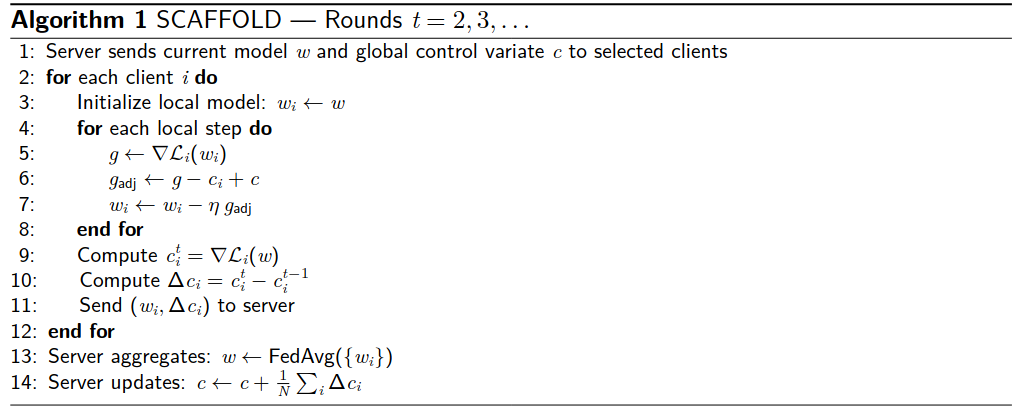
\includegraphics[width=1
    \textwidth]{images/FL7.png}
    \caption{Local Training in Rounds $t \ge 2$}
    \label{fig:MHA2}
\end{figure}

\subsubsection{Take-Home Message}

\textbf{Benefit}:  
SCAFFOLD significantly mitigates client drift by reducing the variance of local updates.
It provably converges faster than FedAvg under partial participation by better aligning
local optimization steps with the global objective.

\textbf{Strengths}:  
Client-side correction substantially improves upon FedAvg’s naive averaging, especially
in challenging non-i.i.d.\ scenarios, leading to faster and more stable convergence.

\textbf{Limitations}:  
Since SCAFFOLD acts only on the client side, it may not be sufficient in highly complex
settings or under extreme heterogeneity. In such cases, additional \textbf{server-side
strategies} may be required to further improve performance.

\section{Prototype-based Approach}

\subsection{Motivation for Prototype Sharing}

Model or gradient averaging methods (e.g., FedAvg-style aggregation) may become suboptimal
when client data distributions are highly heterogeneous. This is particularly evident in
settings where each client observes \textbf{different subsets of classes} or highly
imbalanced class distributions.

In such scenarios, directly averaging model parameters or gradients can lead to
inconsistent updates, since local models may specialize on different classes and develop
very different internal representations. As a result, aggregation at the parameter level
may fail to capture a coherent global structure.

An alternative idea is to share a more \textbf{interpretable intermediate
representation}. Instead of exchanging full models or gradients, clients can communicate
\textbf{class prototypes}, i.e., class-wise feature representations that summarize the
essential characteristics of each class observed locally.

\begin{infobox}[What are class prototypes?]
    A \textbf{class prototype} is a representative feature vector associated with a specific
    class. It is typically computed as the average of the feature embeddings of all samples
    belonging to that class:
    \[
    \mathbf{p}_c
    =
    \frac{1}{|\mathcal{D}_c|}
    \sum_{(x,y)\in\mathcal{D}_c,\; y=c}
    \phi(x),
    \]
    where $\phi(x)$ denotes the feature representation produced by the model and
    $\mathcal{D}_c$ is the set of samples of class $c$.
    
    Class prototypes:
    \begin{compactitemize}
        \item capture the \textbf{semantic essence} of a class in feature space;
        \item are \textbf{compact and interpretable} compared to full model parameters;
        \item can be shared across clients to \textbf{align feature representations} without
        exchanging raw data.
    \end{compactitemize}
\end{infobox}

The underlying hypothesis is that, by sharing and aligning these prototypes, clients can
build a \textbf{consistent global understanding of each class}. This promotes better
generalization across clients and mitigates the negative effects of data heterogeneity,
especially in class-incremental or label-skewed settings.

\subsection{FedProto}

\subsubsection{FedProto Algorithm}

\textbf{FedProto}  is a prototype-based federated learning algorithm designed
to address strong data heterogeneity, especially in scenarios where clients observe
different or non-overlapping sets of classes.

At each communication round, each client $i$ computes a set of \textbf{class prototypes}
$p_{i,c}$, one for each class $c$ present in its local dataset. Given a feature extractor
$f_i$, a classifier $g_i$, and a local dataset $D_i$, the prototype for class $c$ is computed
as:
\[
p_{i,c}
=
\mathbb{E}_{(x,y)\sim D_i}
\bigl[ f_i(x) \;:\; y = c \bigr].
\]

Instead of sending full model parameters or gradients, clients send only their local class
prototypes to the server. The server then aggregates the received prototypes by averaging
them class-wise to obtain a set of \textbf{global prototypes} $\bar{p}_c$ for each class $c$.

\subsubsection{Prototype-Based Regularization}

After aggregation, the server sends the global prototypes back to the clients. Each client
then augments its local training objective with a prototype regularization term:
\[
\mathcal{L}^{\text{FedProto}}_i
=
\mathcal{L}^{\text{local}}_i
+
\lambda
\sum_c
\left\|
p_{i,c} - \bar{p}_c
\right\|_2^2,
\]
which penalizes the discrepancy between the local prototype $p_{i,c}$ and the
corresponding global prototype $\bar{p}_c$.

This regularization encourages the feature representations learned by different clients to
remain \textbf{aligned in feature space}, effectively mitigating the impact of heterogeneous
label distributions.

\subsubsection{Inference}

At inference time, classification can be performed using a \textbf{nearest-mean
classifier}. Given an input sample $x$, the predicted label is:
\[
\hat{y}
=
\arg\min_c
\left\|
f(x) - \bar{p}_c
\right\|_2.
\]

This inference strategy naturally leverages the global prototypes as class representatives
and is particularly effective when class distributions differ across clients.

\subsubsection{Benefits and Empirical Results}

\textbf{Efficiency.}  
Prototype vectors are signiicantly smaller than full model updates, resulting in reduced
communication costs since only prototypes are exchanged instead of entire model
parameters.

\textbf{Effectiveness.}  
By regularizing local representations toward global prototypes, FedProto consistently
outperforms FedAvg and similar aggregation-based methods on heterogeneous benchmarks,
achieving higher accuracy and more stable convergence.

Empirical results show improved handling of scenarios with non-overlapping class
distributions across clients, demonstrating that FedProto enables effective knowledge
sharing beyond raw parameter averaging.

\subsubsection{FedProto Use-Cases}

FedProto is flexible and can be applied in multiple federated learning settings:

\begin{compactitemize}
    \item \textbf{Standard FL:}  
    FedProto can be combined with parameter aggregation methods (e.g., FedAvg) to learn
    a single global model while benefiting from prototype-based alignment.

    \item \textbf{Personalized FL:}  
    Clients can fine-tune their models on local data while sharing knowledge through class
    prototypes, enabling personalization without sacrificing global consistency.

    \item \textbf{Model-Heterogeneous FL:}  
    Since FedProto operates in feature space rather than parameter space, it naturally
    supports scenarios where clients have different model architectures, which makes
    standard parameter-wise aggregation infeasible.
\end{compactitemize}
